Los fundamentos se agrupan según la versión en la que cada herramienta se incorpora al sistema; la
motivación y el alcance de v0, v1 y v2 se establecen en la
Sección~\ref{sec:intro-objetivo-tecnico}.

% ---------------------------------------------------------------
\section{Fundamentos de la versión v0: percepción directa, ROS~2 y salida háptica}
\label{sec:mt-v0}

La versión v0 establece la cadena mínima del sistema: adquirir profundidad con la Intel
RealSense D435i, reducir esa información a una representación compacta, convertirla a
comandos de intensidad háptica y preparar su transmisión hacia el futuro hardware de actuación.
Esta sección presenta los
fundamentos teóricos que sostienen esa primera etapa, desde la sustitución sensorial hasta la
comunicación serie embebida. El objetivo es mostrar cómo una medición densa del entorno
puede convertirse en una señal discreta y de baja latencia sin perder la estructura espacial
necesaria para la asistencia a la movilidad.

\subsection{Sustitución sensorial y neuroplasticidad}
\label{sec:mt-sustitucion}

El principio de sustitución sensorial fue establecido experimentalmente por Bach-y-Rita
et al.\ \cite{BachyRita1969}: una cámara proyectaba patrones de estimulación sobre la espalda
del usuario
mediante una matriz de $20\times20$ actuadores mecánicos, permitiendo a personas ciegas
reconocer objetos y figuras a través del tacto. Este resultado demostró que el cerebro puede
reorganizarse para interpretar señales de modalidades no originales cuando recibe información
espacial consistente, fenómeno conocido como neuroplasticidad sensorial.

Para este trabajo, la relevancia de dicho antecedente es doble. En primer lugar, justifica que
una escena visual pueda codificarse como estímulo háptico si se preserva una correspondencia
espacial estable. En segundo lugar, orienta el diseño hacia representaciones compactas y
repetibles: la interfaz no necesita reconstruir toda la imagen, sino entregar patrones
táctiles consistentes que el usuario pueda aprender a interpretar.

\subsection{Principio físico de la cámara Intel RealSense D435i}
\label{sec:mt-rgbd}

Los sensores RGB-D combinan información visual convencional con una medición de profundidad.
En la familia Intel RealSense D400, y en particular en la D435i, la profundidad se obtiene
mediante estereoscopía infrarroja activa: dos cámaras IR observan la escena y un proyector de
textura facilita la correspondencia entre vistas en regiones con bajo contraste
\cite{RS-D400,IntelRealSenseDepthTuning}. El resultado es una imagen de profundidad $D(u,v)$ donde
cada píxel codifica la distancia al plano de la cámara; los valores centinela $D=0$ y
$D=65535$ indican ausencia de medición válida.

Bajo imágenes rectificadas, la correspondencia entre un píxel de la vista izquierda $u_L$ y
el píxel correspondiente de la vista derecha $u_R$ define la disparidad $d=u_L-u_R$. Aplicando
semejanza de triángulos en el sistema estereoscópico se obtiene:
\begin{equation}
  Z = \frac{f\,B}{d},
  \label{eq:stereo-depth}
\end{equation}
donde $Z$ es la profundidad, $f$ la distancia focal en píxeles y $B$ la separación entre
cámaras
\cite{Hartley2004,Scharstein2002}. La ecuación~\ref{eq:stereo-depth} muestra que el error de
profundidad crece al disminuir la disparidad, por lo que las mediciones lejanas son más
sensibles al ruido y a errores de correspondencia.

La D435i publica, además de la imagen de profundidad, flujos de color, profundidad alineada a
color, parámetros intrínsecos de cámara y señales inerciales. En v0 se utiliza
principalmente la imagen de profundidad rectificada y su \texttt{CameraInfo}. En v1 se
incorpora la IMU a través del acelerómetro, no para estimar desplazamiento, sino para obtener
la dirección de la gravedad y estabilizar la nube antes de detectar el suelo. En v2 se agregan
la imagen RGB, la profundidad alineada a color y la orientación IMU filtrada; en esta etapa
también se utiliza el giróscopo, integrado por el filtro de Madgwick, como apoyo de
\texttt{rgbd\_odometry}.

\subsection{Modelo de cámara \emph{pinhole} y proyección inversa}
\label{subsec:mt-pinhole}

El procesamiento geométrico se apoya en el modelo \emph{pinhole}. Un punto
$\mathbf{P}=(X,Y,Z)^T$ expresado en el marco de la cámara se proyecta al píxel $(u,v)$
mediante:
\begin{equation}
  \begin{pmatrix} u \\ v \\ 1 \end{pmatrix}
  = \frac{1}{Z}\,K\,\begin{pmatrix} X \\ Y \\ Z \end{pmatrix}, \qquad
  K =
  \begin{pmatrix}
    f_x & 0 & c_x \\
    0 & f_y & c_y \\
    0 & 0 & 1
  \end{pmatrix}.
  \label{eq:pinhole}
\end{equation}
En la ecuación~\ref{eq:pinhole}, $f_x$ y $f_y$ son las distancias focales en píxeles,
mientras que $(c_x,c_y)$ es el centro de proyección. La operación inversa, necesaria para
reconstruir una nube 3D a partir de una imagen de profundidad, queda:
\begin{equation}
  X = \frac{(u-c_x)\,Z}{f_x}, \qquad
  Y = \frac{(v-c_y)\,Z}{f_y}, \qquad
  Z = D(u,v)\times 10^{-3}\,\text{m}.
  \label{eq:pinhole-inv}
\end{equation}
Los parámetros de $K$ se obtienen del mensaje \texttt{sensor\_msgs/CameraInfo}, lo que evita
fijar intrínsecos a mano y mantiene coherencia con el perfil activo de resolución y
calibración
\cite{Hartley2004}.

\subsection{Limitaciones por superficies especulares e iluminación intensa}
\label{subsec:mt-depth-reflections}

La estimación estéreo supone que los píxeles comparados en ambas cámaras observan el mismo
punto físico mediante trayectorias ópticas directas y que su apariencia local es
suficientemente similar. Esta hipótesis se cumple razonablemente bien en superficies difusas,
pero se debilita en superficies especulares o semiespeculares, como pisos pulidos, baldosas
brillantes, metal, vidrio o zonas húmedas. En esos casos la energía infrarroja emitida por el
proyector de textura, o la luz proveniente de una fuente externa, se refleja de manera
direccional y puede llegar a cada cámara desde caminos ópticos distintos.

El problema no es solamente la ausencia de datos. Si el algoritmo de correspondencia no
encuentra textura confiable o detecta saturación, el resultado esperable es una medición
inválida. Sin embargo, también puede ocurrir una correspondencia falsa pero internamente
consistente. Un reflejo sobre el piso puede aparecer en ambas cámaras IR con posiciones
compatibles con cierta disparidad $d$; al aplicar la ecuación~\ref{eq:stereo-depth}, el
sistema interpreta esa disparidad como una profundidad real, aunque el patrón observado
corresponda a una reflexión, a una imagen virtual o a luz parásita.

Al retroproyectar mediante la ecuación~\ref{eq:pinhole-inv}, esa medición se convierte en un
punto 3D que no pertenece a un obstáculo físico. Para una interfaz háptica, este fenómeno
tiende a manifestarse como falso positivo si la agregación por celda conserva una lectura
cercana aislada. La mitigación requiere tratar estas lecturas como una limitación física del
sensor y no como un error puramente algorítmico: descartar inválidos, exigir soporte espacial
mínimo, incorporar persistencia temporal y verificar coherencia con el plano de suelo
\cite{RS-D400,IntelRealSenseDepthTuning}.

\subsection{ROS~2 como middleware de integración}
\label{sec:mt-ros2}

ROS~2 organiza un sistema robótico como un grafo de nodos que intercambian mensajes tipados
mediante tópicos, servicios y acciones \cite{ROS}. En este trabajo se utiliza principalmente
el patrón publicador-suscriptor: cada etapa produce una representación intermedia y la
siguiente la consume sin depender de la implementación interna del productor. Este
desacoplamiento permite separar adquisición, percepción, mapeo, visualización y salida al
hardware.

La comunicación en ROS~2 se apoya en DDS. Esto habilita ejecutar el procesamiento principal en
la Raspberry Pi y visualizar resultados en otra computadora dentro de la misma red, siempre que
ambas participen del mismo dominio DDS. Además, los remapeos permiten adaptar nombres de
tópicos en el lanzamiento sin introducir nodos adicionales. Esta propiedad es importante para
la D435i, cuyo driver publica nombres nativos extensos, mientras que los nodos propios consumen
interfaces normalizadas.

La teoría relevante para v0 no es solamente la existencia de tópicos, sino la elección de
mensajes. Una imagen de profundidad se transporta como \texttt{sensor\_msgs/Image}, los
parámetros intrínsecos como \texttt{sensor\_msgs/CameraInfo}, la grilla compacta como
\texttt{DepthGrid} y la salida lógica de intensidades como \texttt{HapticGrid}. Al definir mensajes
explícitos se evita codificar semántica en arreglos sin contexto y se preserva trazabilidad
entre nodos.

\subsection{Reducción espacial del mapa de profundidad}
\label{sec:mt-depth-grid-encoder}

Un mapa de profundidad a resolución nativa contiene cientos de miles de píxeles por frame,
pero esa densidad no puede trasladarse de forma directa a una interfaz háptica corporal. La
limitación principal no es solamente computacional o de transmisión, sino perceptual: el
usuario no puede distinguir de manera confiable estímulos hápticos arbitrariamente cercanos
ni interpretar una matriz demasiado densa como si fuera una imagen visual. Por este motivo, la
escena debe reducirse a una representación espacial de baja dimensión que conserve la
ubicación aproximada y la urgencia de los obstáculos. En v0, esta reducción se realiza
particionando la imagen en regiones de interés y calculando estadísticas por región.

La imagen de dimensiones $W\times H$ se divide en una grilla de $R\times C$ regiones de
interés (ROI). Las fronteras de cada ROI se calculan mediante división entera uniforme:
\begin{equation}
  x_c^{(k)} = \left\lfloor \frac{k\,W}{C} \right\rfloor,\quad k=0,\ldots,C;
  \qquad
  y_r^{(j)} = \left\lfloor \frac{j\,H}{R} \right\rfloor,\quad j=0,\ldots,R.
  \label{eq:roi-edges}
\end{equation}
La ecuación~\ref{eq:roi-edges} distribuye el error de cuantización entre celdas, de modo que
regiones adyacentes difieran a lo sumo en un píxel \cite{gonzalez2018digital}.

Para cada ROI$(r,c)$ se recorren los píxeles válidos dentro del rango $[z_{\min},z_{\max}]$ y
se acumulan:
\begin{equation}
  \bar{z}_{r,c} =
  \frac{1}{N_{r,c}}\sum_{(u,v)\in\text{ROI}_{r,c}} z_{u,v},
  \qquad
  z^{\min}_{r,c} = \min_{(u,v)} z_{u,v},
  \qquad
  N_{r,c} = \#\{\text{píxeles válidos}\}.
  \label{eq:cell-stats}
\end{equation}
Junto con el máximo $z^{\max}_{r,c}$, estas estadísticas permiten distinguir ausencia de
medición, obstáculo cercano y distribución de profundidad dentro de una región. El mínimo
es conservador porque preserva el obstáculo más cercano, mientras que la media atenúa
píxeles aislados
\cite{hornung2013octomap}.

\subsection{Codificación angular de la nube filtrada}
\label{sec:mt-angular-grid}

Aunque v0 reduce directamente la imagen de profundidad en ROIs de imagen, las versiones v1 y v2
construyen la grilla a partir de una nube de obstáculos ya filtrada. En ese caso, la
partición horizontal puede definirse en ángulo, no solo en coordenada de imagen. Si un punto
tiene coordenadas $(x,z)$ en el plano horizontal de la cámara, su ángulo lateral es:
\begin{equation}
  \beta = \operatorname{atan2}(x,z).
  \label{eq:angular-bin-angle}
\end{equation}
La apertura horizontal activa se divide en columnas, y cada punto se asigna a la columna
correspondiente según $\beta$. La distancia usada para codificar proximidad es radial:
\begin{equation}
  d = \sqrt{x^2+z^2}.
  \label{eq:radial-distance}
\end{equation}
La ecuación~\ref{eq:radial-distance} evita subestimar obstáculos laterales: usar solo $z$
puede hacer que dos obstáculos con distinta separación lateral parezcan equivalentes si
comparten la misma componente frontal.

\subsection{Mapeo de distancia a comando de intensidad}
\label{sec:mt-dist-to-intensity}

Para traducir la distancia por celda a una señal háptica se emplea una función lineal
invertida y saturada. La proximidad del obstáculo debe producir mayor intensidad, con
saturación en los extremos del rango útil:
\begin{equation}
  I_i =
  \begin{cases}
    I_{\max} & \text{si } z^{\min}_i \leq z_{\min}, \\
    0        & \text{si } z^{\min}_i \geq z_{\max}, \\
    \dfrac{z_{\max} - z^{\min}_i}{z_{\max} - z_{\min}}
    \cdot I_{\max} & \text{en otro caso.}
  \end{cases}
  \label{eq:intensity-mapping}
\end{equation}
En la ecuación~\ref{eq:intensity-mapping}, $z_{\min}$ y $z_{\max}$ delimitan el rango de
operación, $I_{\max}$ es la intensidad máxima e $I_i$ es la intensidad lógica asociada a la celda
$i$. Esta conversión se realiza en \texttt{haptic\_grid\_generator}; las celdas sin medición válida
permanecen inactivas.

La intensidad lógica no es todavía el ciclo de trabajo aplicado a un motor. La interfaz UART
posterior limita $I_i$ al intervalo $[0,100]$ y la escala mediante el máximo configurado
$D_{\max}$:
\begin{equation}
  D_i =
  \begin{cases}
    \left\lfloor
      \dfrac{
        \operatorname{round}\!\left(\operatorname{sat}_{[0,100]}(I_i)\right)
        D_{\max}
      }{100}
    \right\rfloor, & \text{si la celda está activa},\\
    0, & \text{si la celda está inactiva}.
  \end{cases}
  \label{eq:duty-scaling}
\end{equation}
Esta segunda operación no vuelve a interpretar la distancia: solo adapta el comando ya calculado
al límite de salida y lo prepara para su serialización.

\subsection{Comunicación serie embebida}
\label{sec:mt-uart}

La transmisión prevista entre la computadora de placa simple y el futuro controlador de actuación
requiere definir un protocolo de enlace. UART
(\emph{Universal Asynchronous Receiver-Transmitter}) es
una opción habitual en sistemas embebidos por su disponibilidad y simplicidad.
En modo 8N1, cada byte requiere 10 bits físicos: un bit de inicio,
ocho bits de datos y un bit de parada. Por lo tanto, para una trama de longitud
$L_{\text{trama}}$ y baudrate $B$:
\begin{equation}
  t_{\text{tx}} = \frac{10\cdot L_{\text{trama}}}{B}.
  \label{eq:uart-time}
\end{equation}
La ecuación~\ref{eq:uart-time} permite verificar que la transmisión no comprometa el período
del lazo háptico.

Existen dos enfoques de codificación. En ASCII, los valores se representan como caracteres
decimales separados por espacios y terminados con \texttt{\textbackslash n}; es legible y
fácil de depurar, pero menos eficiente. En binario compacto, cada intensidad puede codificarse
en un \texttt{uint8}; al agregar longitud y CRC-8 se obtiene una trama más robusta y eficiente
\cite{smbus2000}. En la configuración actual, el formato ASCII de tipo \texttt{M $D_0$ $D_1$
... $D_{N-1}$\textbackslash n} resulta suficiente para una matriz de 5 filas $\times$ 10 columnas a
$115200\,\text{bps}$, mientras que un formato binario queda como alternativa natural para
matrices de mayor densidad.

En esta tesis se implementan la construcción y la transmisión de la trama, pero no su recepción ni
la conversión de los valores transmitidos en estímulos físicos. El microcontrolador receptor, la
electrónica de potencia y los actuadores pertenecen a la segunda etapa del proyecto.

% ---------------------------------------------------------------
\section{Fundamentos de la versión v1: orientación, gravedad y suelo}
\label{sec:mt-v1}

La versión v1 parte de la solución funcional establecida en v0 y conserva su salida compacta, pero
mejora la interpretación previa de las mediciones al modificar la fuente de la grilla: en
lugar de codificar profundidad cruda, primero proyecta la imagen a una nube 3D, la alinea con
la gravedad y separa suelo, obstáculos y techo. La teoría de esta etapa combina
representaciones de orientación, filtrado inercial y estimación robusta de planos. En esta
versión no se utiliza Madgwick de forma deliberada: la decisión de diseño es estimar
solamente la vertical necesaria para remover el suelo, evitando incorporar una estimación
completa de orientación cuando no aporta a la salida háptica y puede aumentar latencia,
dependencias y costo computacional.

\subsection{Ángulos de cámara y convención óptica}
\label{sec:mt-camera-angles}

La orientación de la cámara puede describirse mediante ángulos de Euler: \emph{roll} ($\phi$),
\emph{pitch} ($\theta$) y \emph{yaw} ($\psi$). En la convención óptica de la D435i, $x$
apunta hacia la derecha de la imagen, $y$ hacia abajo y $z$ hacia adelante. En esa convención, roll
corresponde a la rotación alrededor de $z$, pitch alrededor de $x$ e yaw alrededor de $y$,
como se muestra en la Figura~\ref{fig:euler-angles}.

\begin{figure}[ht]
  \centering
  \begin{minipage}[b]{0.32\textwidth}
    \centering
    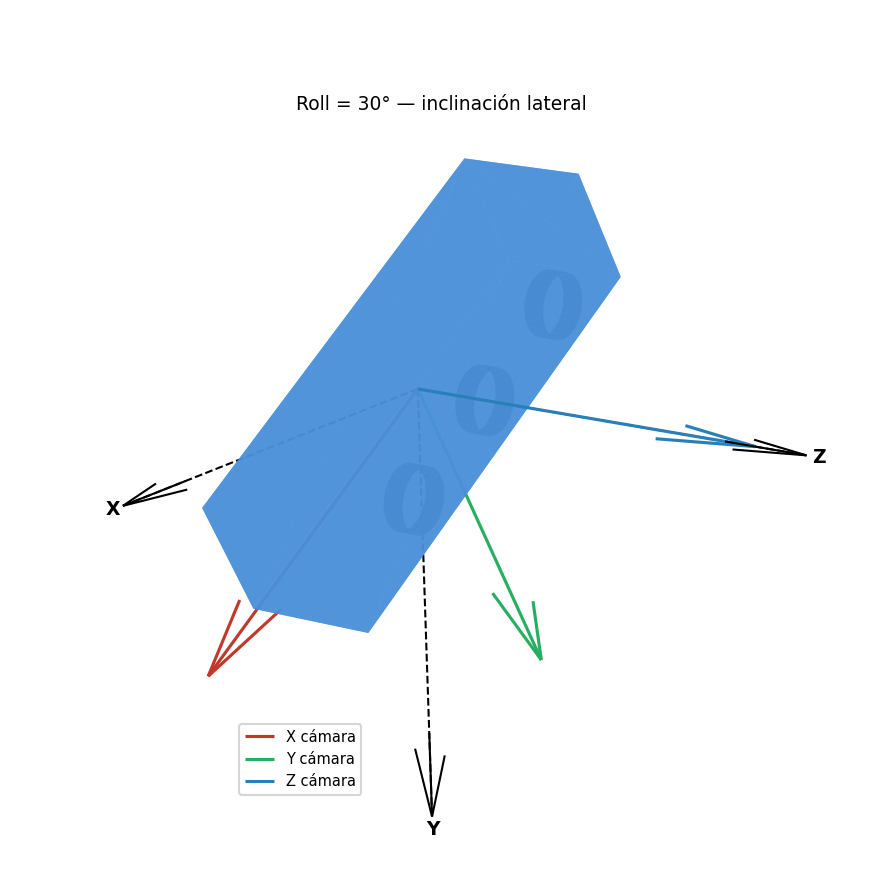
\includegraphics[width=\textwidth]{_Imagenes/local_mapper/roll_30.png}
    \subcaption{Roll $=30^\circ$: rotación alrededor de $z$.}
    \label{fig:cam-roll-30}
  \end{minipage}
  \hfill
  \begin{minipage}[b]{0.32\textwidth}
    \centering
    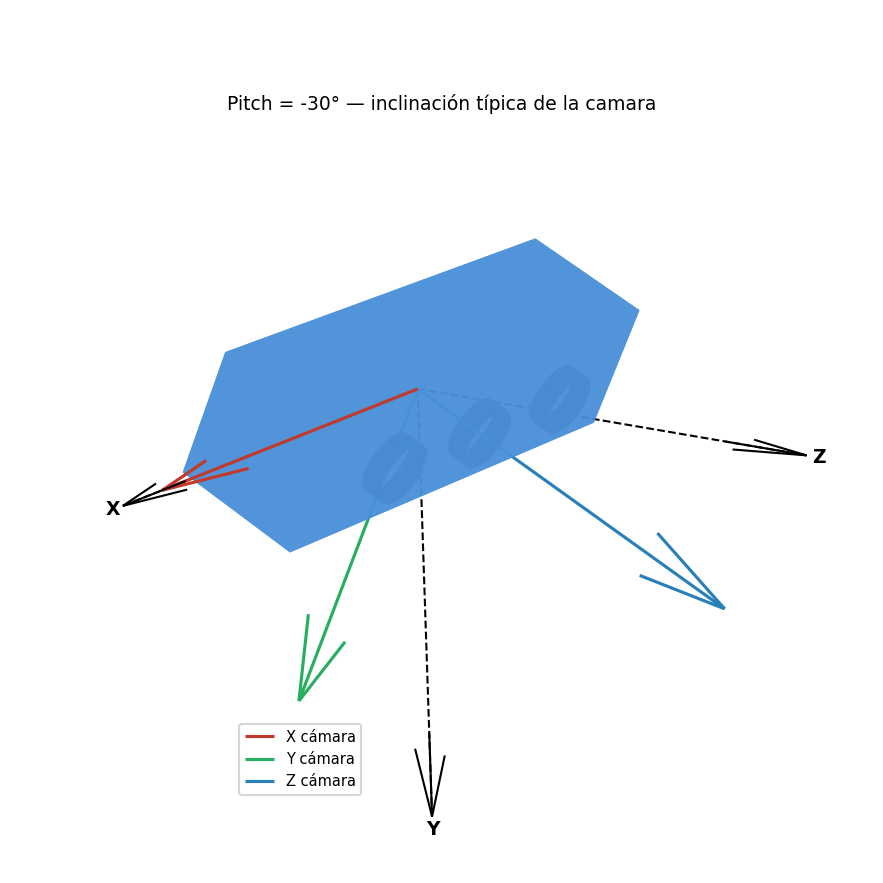
\includegraphics[width=\textwidth]{_Imagenes/local_mapper/pitch_n30.png}
    \subcaption{Pitch $=-30^\circ$: rotación alrededor de $x$.}
    \label{fig:cam-pitch-30}
  \end{minipage}
  \hfill
  \begin{minipage}[b]{0.32\textwidth}
    \centering
    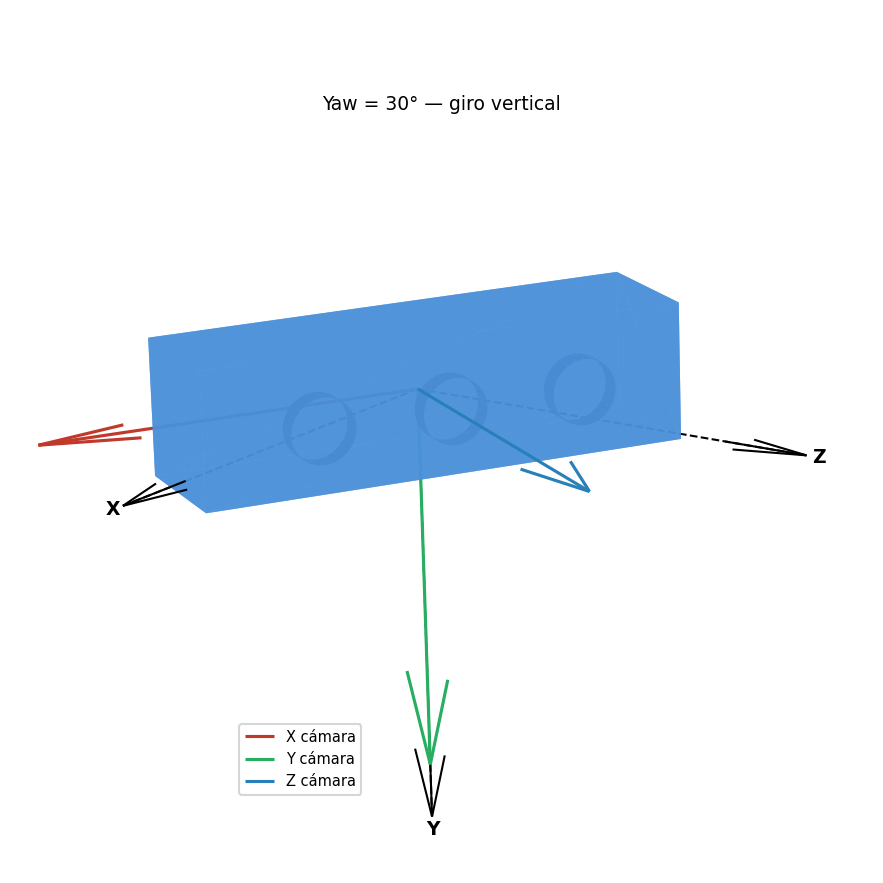
\includegraphics[width=\textwidth]{_Imagenes/local_mapper/yaw_30.png}
    \subcaption{Yaw $=30^\circ$: rotación alrededor de $y$.}
    \label{fig:cam-yaw-30}
  \end{minipage}
  \caption{Ángulos de Euler en la convención óptica de la cámara. Cada rotación se
    representa alrededor de un eje fijo del sensor.}
  \label{fig:euler-angles}
\end{figure}

La Figura~\ref{fig:euler-angles} también permite distinguir dos funciones diferentes. Roll y
pitch modifican la relación entre la nube y el plano de suelo, por lo que deben compensarse
antes de segmentar. En cambio, yaw rota la cámara alrededor de la vertical y no cambia qué
puntos pertenecen al suelo; su importancia aparece en v2, cuando se acumulan observaciones en
un marco común.

\subsection{Singularidad de Euler y cuaterniones}
\label{sec:mt-quaternions}

Los ángulos de Euler presentan una singularidad conocida como \emph{gimbal lock}: cuando
$\theta=\pm90^\circ$, dos ejes de rotación quedan alineados y se pierde un grado de libertad.
La Figura~\ref{fig:cam-gimbal} muestra una configuración alcanzable cuando la cámara apunta
casi verticalmente hacia abajo.

\begin{figure}[ht]
  \centering
  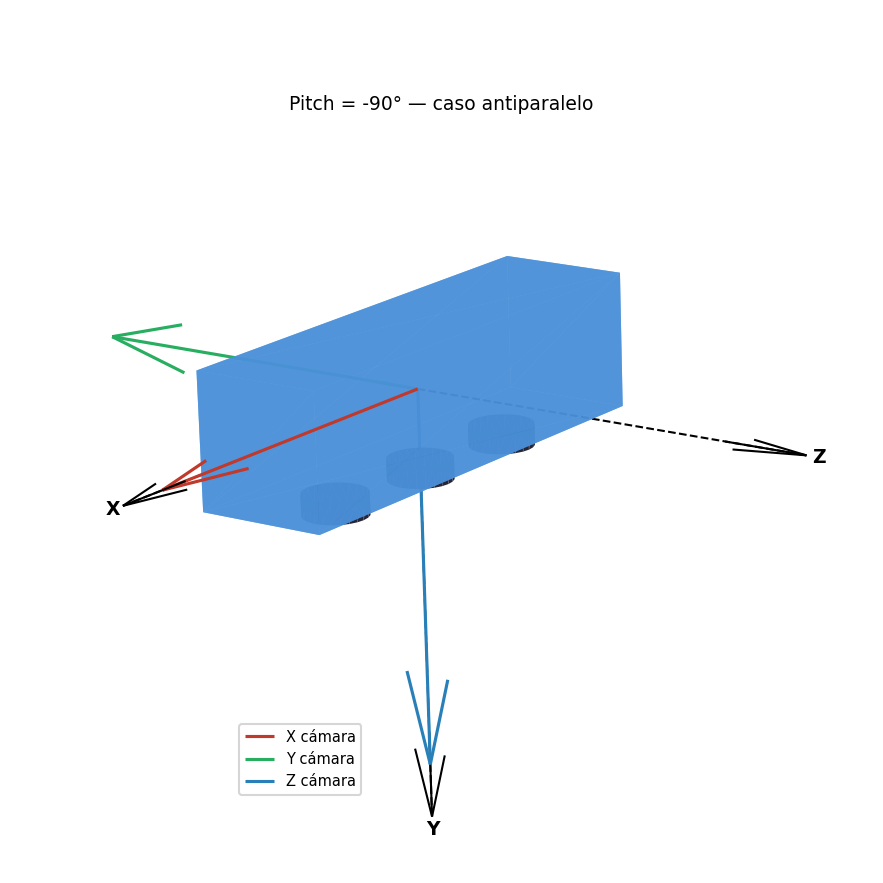
\includegraphics[width=0.45\textwidth]{_Imagenes/local_mapper/pitch_n90.png}
  \caption{Singularidad \emph{gimbal lock}: con pitch $=-90^\circ$ la cámara apunta
    verticalmente hacia abajo y los ejes de roll y yaw quedan alineados.}
  \label{fig:cam-gimbal}
\end{figure}

Para evitar esa singularidad se usa una representación mediante cuaterniones unitarios. Un
cuaternión se define como:
\begin{equation}
  q = q_w + q_x\,\mathbf{i} + q_y\,\mathbf{j} + q_z\,\mathbf{k},
  \label{eq:quat-def-mt}
\end{equation}
donde $q_w$ es la parte escalar y $(q_x,q_y,q_z)^T$ la parte vectorial. Si $\lVert q\rVert=1$,
representa una rotación de ángulo $\theta$ alrededor de un eje unitario $\hat{\mathbf{n}}$:
\begin{equation}
  q = \left(\cos\frac{\theta}{2},\; \hat{\mathbf{n}}\sin\frac{\theta}{2}\right).
  \label{eq:quat-unit-mt}
\end{equation}
La rotación de un punto $\mathbf{p}$ se expresa como
$\mathbf{p}'=q\otimes(0,\mathbf{p})\otimes q^*$, donde $q^*$ es el conjugado. La
Figura~\ref{fig:quat-orientations} muestra las poses resultantes junto con el cuaternión
unitario que las representa: a la izquierda, una composición de roll y pitch; a la derecha,
una configuración singular para Euler donde distintas ternas angulares pueden describir la
misma orientación física.

\begin{figure}[ht]
  \centering
  \begin{minipage}[b]{0.48\textwidth}
    \centering
    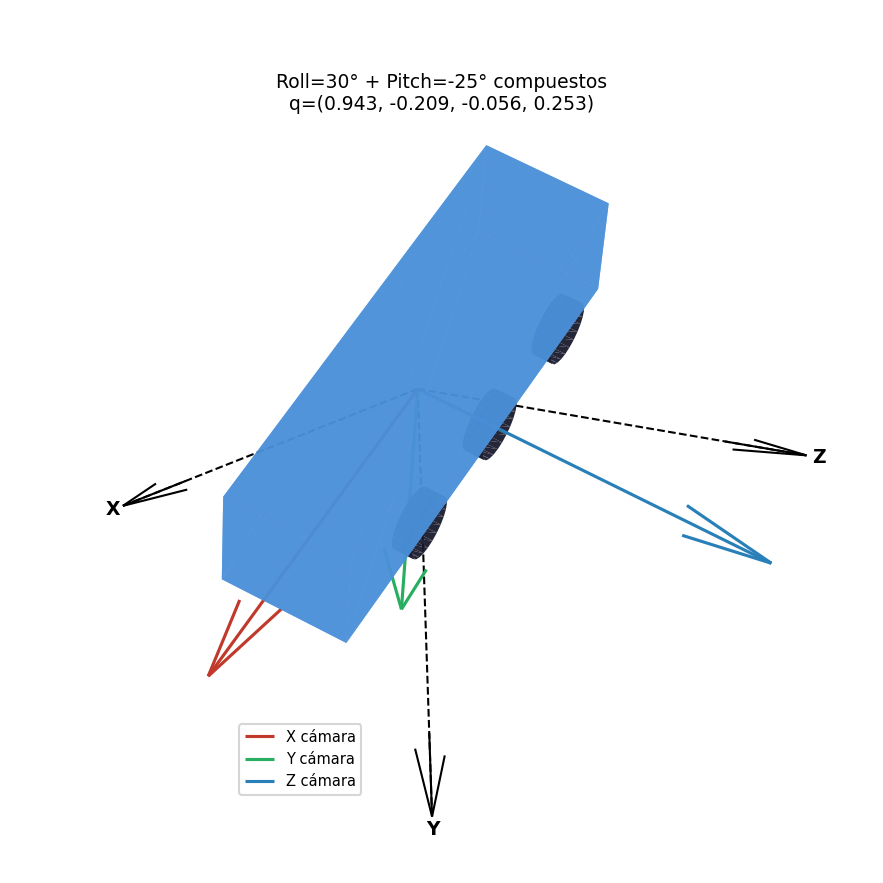
\includegraphics[width=\textwidth]{_Imagenes/local_mapper/roll30_pitch_n25.png}
    \subcaption{Roll y pitch compuestos en un único cuaternión.}
    \label{fig:cam-quat-composed}
  \end{minipage}
  \hfill
  \begin{minipage}[b]{0.48\textwidth}
    \centering
    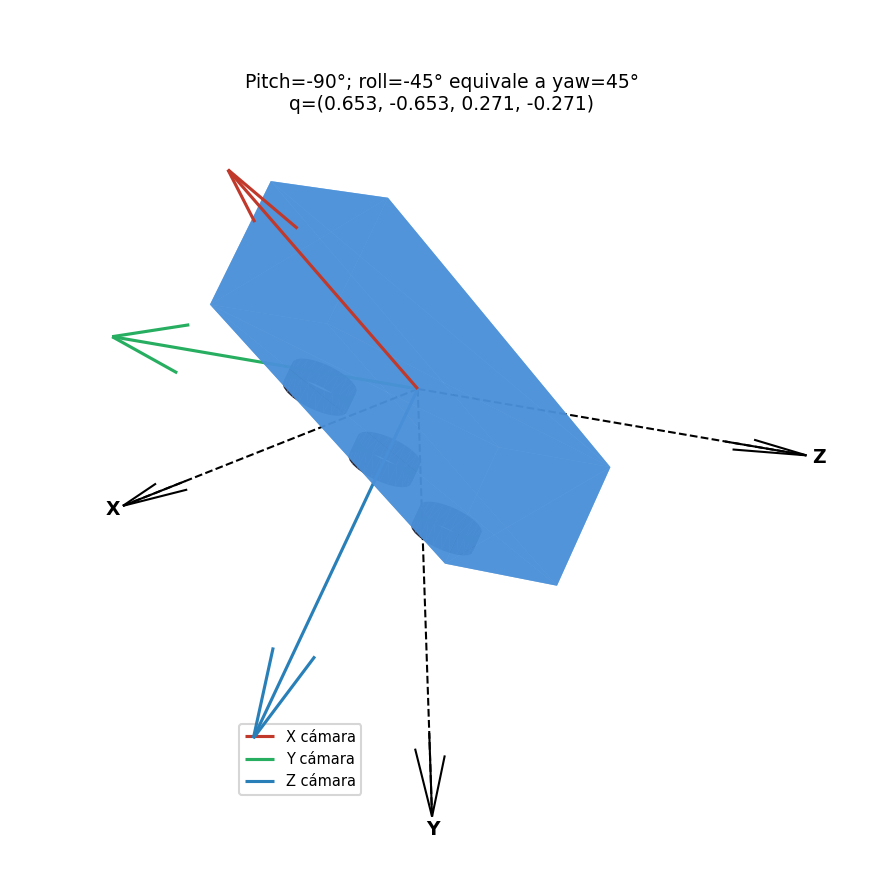
\includegraphics[width=\textwidth]{_Imagenes/local_mapper/gimbal_lock_ambiguous.png}
    \subcaption{Orientación en la singularidad de Euler.}
    \label{fig:cam-quat-gimbal-ambiguous}
  \end{minipage}
  \caption{Ventajas de la representación mediante cuaterniones para orientaciones compuestas
    y configuraciones singulares.}
  \label{fig:quat-orientations}
\end{figure}

\subsection{Alineación gravitacional con acelerómetro}
\label{sec:mt-imu}

La IMU de la D435i incluye acelerómetro y giróscopo de tres ejes \cite{RS-D400}. En v1, el
acelerómetro se usa para estimar la dirección de la gravedad. Esta elección evita integrar
el giróscopo o ejecutar un filtro de orientación completo: para detectar suelo alcanza con conocer
roll y pitch respecto de la vertical, mientras que yaw no modifica la altura de los puntos ni
la coplanaridad del piso. En reposo, en el frame óptico de la cámara, una cámara horizontal
mide aproximadamente $\mathbf{a}=(0,-g,0)$, como se muestra en la
Figura~\ref{fig:cam-horizontal}.

\begin{figure}[ht]
  \centering
  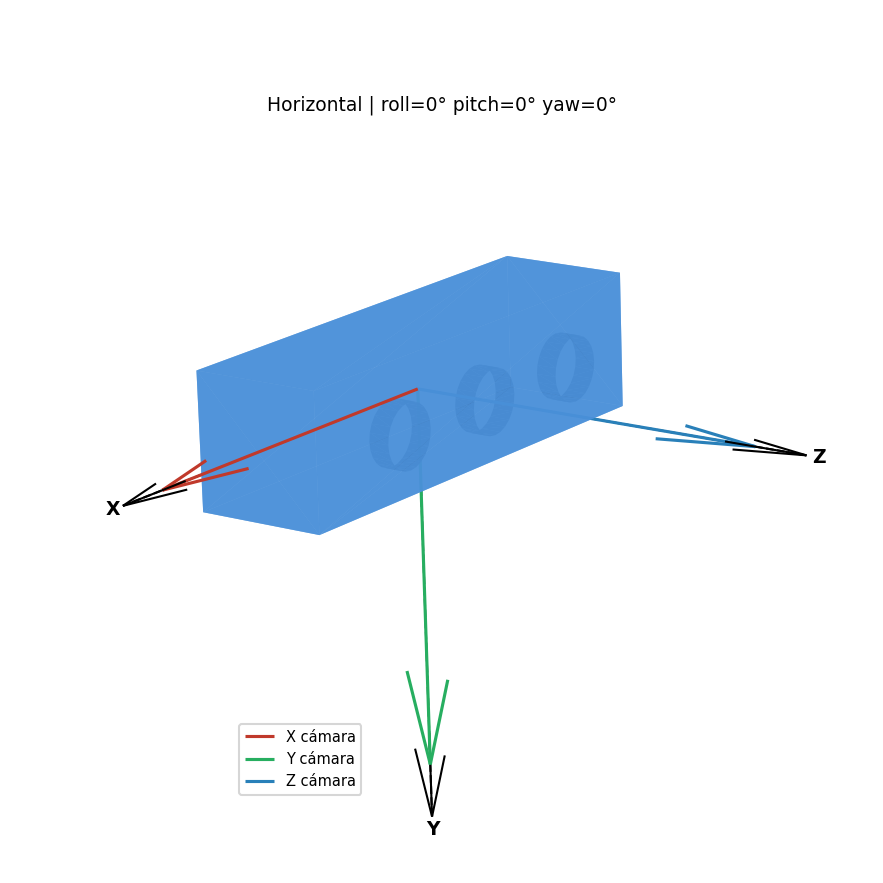
\includegraphics[width=0.45\textwidth]{_Imagenes/local_mapper/horizontal.png}
  \caption{Cámara D435i en posición horizontal. El acelerómetro mide $(0,-g,0)$ en la
    convención óptica usada por el pipeline.}
  \label{fig:cam-horizontal}
\end{figure}

A partir de $\mathbf{a}=(a_x,a_y,a_z)^T$ pueden estimarse roll y pitch sin integración
temporal:
\begin{equation}
  \phi = \operatorname{atan2}(a_y,a_z),
  \qquad
  \theta = \operatorname{atan2}\!\left(-a_x,\sqrt{a_y^2+a_z^2}\right).
  \label{eq:accel-roll-pitch}
\end{equation}
La ecuación~\ref{eq:accel-roll-pitch} no estima yaw, ya que la gravedad no contiene
información sobre rotación alrededor de la vertical. Para construir el marco alineado a
gravedad se calcula la rotación mínima que lleva el vector de aceleración normalizado
$\hat{\mathbf{a}}$ al vector canónico $\hat{\mathbf{b}}=(0,-1,0)$. En forma proporcional:
\begin{align}
  q_w &= 1 + \hat{\mathbf{a}}\cdot\hat{\mathbf{b}}, \label{eq:qmin-w-mt}\\
  \mathbf{q}_v &= \hat{\mathbf{a}}\times\hat{\mathbf{b}}. \label{eq:qmin-v-mt}
\end{align}
Luego se normaliza $q\leftarrow q/\lVert q\rVert$. La Figura~\ref{fig:rot-min-cases} muestra el
caso identidad y el caso antiparalelo, donde el eje queda indeterminado y debe resolverse de
forma explícita.

\begin{figure}[ht]
  \centering
  \begin{minipage}[b]{0.48\textwidth}
    \centering
    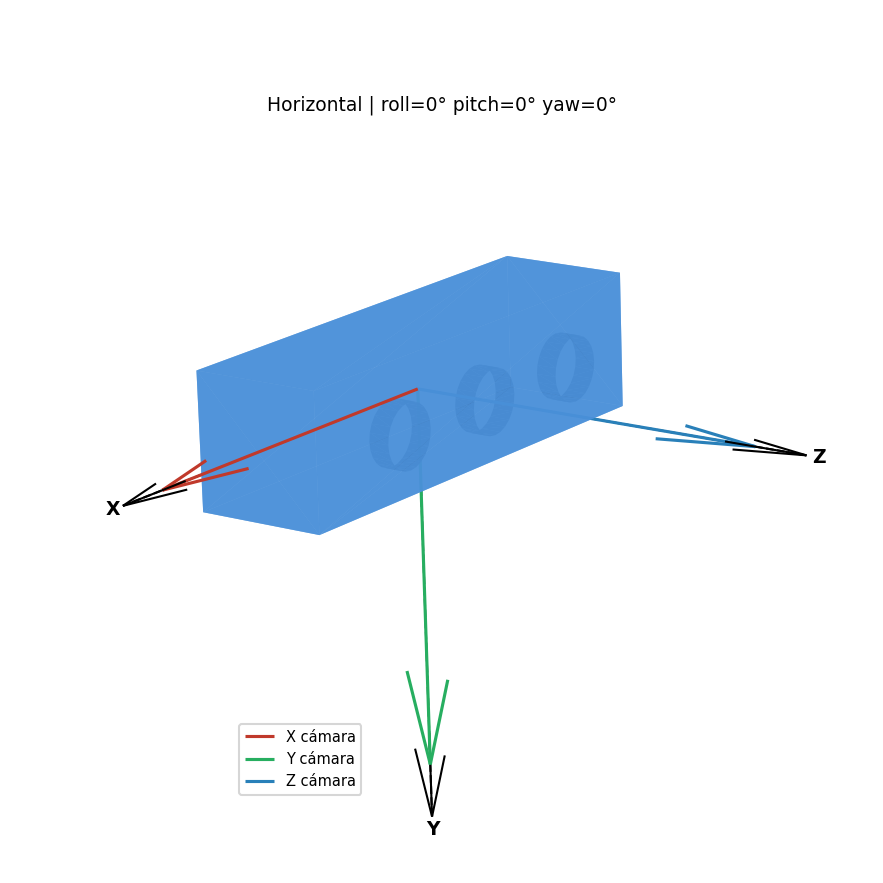
\includegraphics[width=\textwidth]{_Imagenes/local_mapper/horizontal.png}
    \subcaption{Caso identidad: $\hat{\mathbf{a}}=\hat{\mathbf{b}}$.}
    \label{fig:rot-min-identity}
  \end{minipage}
  \hfill
  \begin{minipage}[b]{0.48\textwidth}
    \centering
    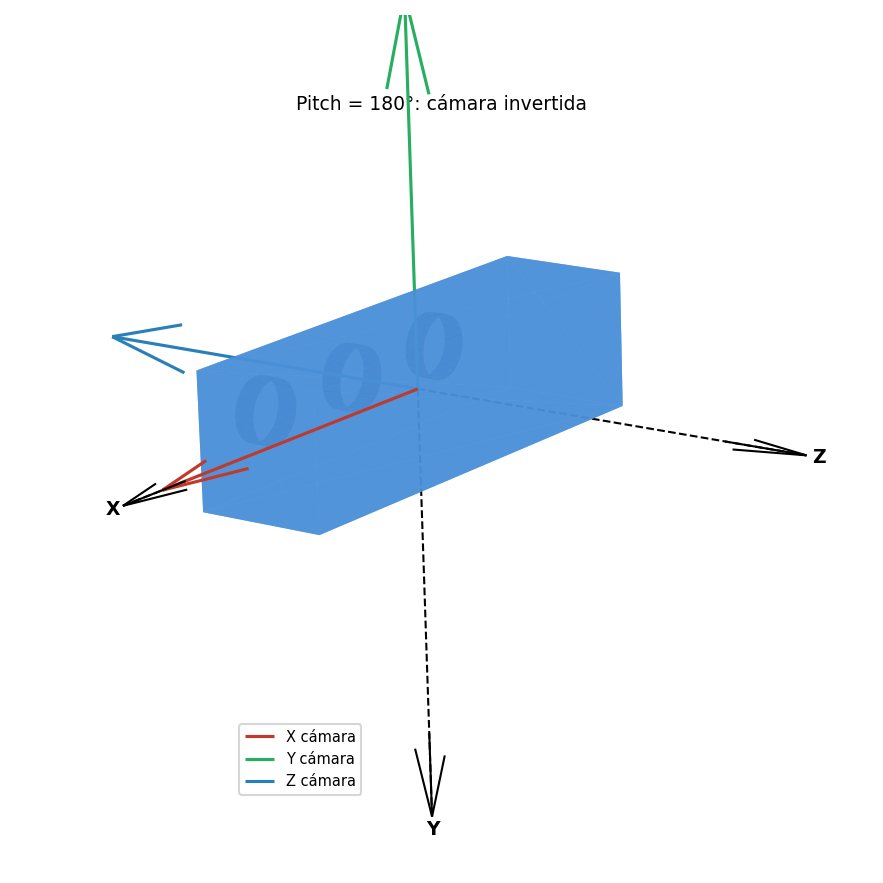
\includegraphics[width=\textwidth]{_Imagenes/local_mapper/pitch_180.png}
    \subcaption{Caso antiparalelo: $\hat{\mathbf{a}}=-\hat{\mathbf{b}}$.}
    \label{fig:rot-min-antiparallel}
  \end{minipage}
  \caption{Casos límite en el cálculo de la rotación mínima entre el vector de
    aceleración y la vertical canónica.}
  \label{fig:rot-min-cases}
\end{figure}

\subsection{Filtrado inercial local para la dirección de gravedad}
\label{sec:mt-accel-filter}

El acelerómetro no mide únicamente gravedad. Durante la marcha registra aceleraciones
lineales de la cabeza, vibraciones y golpes \cite{menz2003acceleration,Woodman2007}. Por eso,
antes de usarlo como referencia vertical se aplica un filtro IIR pasa bajos de primer orden:
\begin{equation}
  \mathbf{a}_f[k] = \alpha\,\mathbf{a}[k] + (1-\alpha)\,\mathbf{a}_f[k-1].
  \label{eq:iir-accel}
\end{equation}
La constante usada en el código, $\alpha\approx0{,}136$, corresponde a una frecuencia de corte
aproximada de $5\,\text{Hz}$ con una tasa de muestreo cercana a $200\,\text{Hz}$
\cite{oppenheim1999dsp}. Además, se descartan muestras cuya norma supera $2{,}5g$ y se activa un
indicador de dinámica cuando la norma filtrada se aleja más de $0{,}5\,\text{m/s}^2$ de $g$.
Este esquema permite estabilizar la vertical sin depender de la odometría ni de un filtro de
orientación completo, manteniendo el procesamiento de v1 acotado para tiempo real.

\subsection{Integración de giróscopo y deriva de yaw}
\label{sub:mt-heading}

El giróscopo mide velocidad angular. Si se integra la componente asociada al eje vertical, el
yaw evoluciona como:
\begin{equation}
  \psi(t) = \psi(t-\Delta t) + \omega_y(t)\,\Delta t.
  \label{eq:heading-integration}
\end{equation}
La ecuación~\ref{eq:heading-integration} permite entender la deriva: un sesgo constante del
giróscopo produce error angular acumulativo \cite{Woodman2007}. En v1, este yaw no es
necesario para segmentar suelo; en v2, la orientación horizontal se corrige mediante
odometría visual-inercial.

\subsection{Detección del plano del suelo}
\label{sec:mt-ground-detection}

Una vez que la nube está alineada a gravedad, el suelo aparece como un conjunto de puntos
coplanares a una altura aproximadamente constante. Un plano se representa mediante:
\begin{equation}
  \mathbf{n}\cdot\mathbf{p}+d=0,
  \label{eq:plane-implicit}
\end{equation}
donde $\mathbf{n}$ es la normal unitaria y $d$ la distancia con signo al origen. La distancia
con signo de un punto $\mathbf{q}$ al plano es:
\begin{equation}
  \delta(\mathbf{q}) = \mathbf{n}\cdot\mathbf{q}+d.
  \label{eq:point-plane-dist}
\end{equation}
La ecuación~\ref{eq:point-plane-dist} permite clasificar puntos según su separación respecto
del plano estimado.

\subsection{Estimación adaptativa de ruido}
\label{subsec:mt-nn-noise}

El ruido de profundidad depende de la distancia y de la reflectividad. Para adaptar la
tolerancia de inliers, se estima la distancia media al vecino más cercano sobre un subconjunto
de la nube
\cite{gonzalez2018digital}:
\begin{equation}
  \bar{d}_{NN} =
  \frac{1}{m}\sum_{i=1}^{m}\min_{j\neq i}\lVert\mathbf{p}_i-\mathbf{p}_j\rVert.
  \label{eq:nn-dist}
\end{equation}
La desviación estándar de esa distribución, $\sigma_{NN}$, aproxima el ruido puntual. Bajo
una hipótesis gaussiana, una tolerancia $\varepsilon=3\sigma_{NN}$ cubre el $99{,}7\,$\% de
las mediciones esperadas para puntos del plano, con cotas inferiores y superiores para evitar
inestabilidad numérica:
\begin{equation}
  \varepsilon = 3\,\sigma_{NN}.
  \label{eq:adaptive-tol}
\end{equation}

\subsection{Submuestreo por voxel grid}
\label{subsec:mt-voxel}

Una nube a plena resolución puede contener cientos de miles de puntos. Como el conteo de
inliers de RANSAC escala linealmente con la cantidad de puntos, una estrategia habitual de
reducción es el submuestreo por \emph{voxel grid}: el espacio se divide en celdas cúbicas de
lado $s$ y cada punto $\mathbf{p}_i=(x_i,y_i,z_i)$ se asigna a la clave discreta
\[
  \mathbf{k}_i =
  \left(\left\lfloor \frac{x_i}{s} \right\rfloor,
        \left\lfloor \frac{y_i}{s} \right\rfloor,
        \left\lfloor \frac{z_i}{s} \right\rfloor\right).
\]
Los puntos que caen en una misma celda $V_{\mathbf{k}}$ se reemplazan por un único
representante. En la implementación analizada, dicho representante es el promedio aritmético
por coordenada,
\[
  \bar{\mathbf{p}}_{\mathbf{k}} =
  \frac{1}{N_{\mathbf{k}}}
  \sum_{\mathbf{p}_i \in V_{\mathbf{k}}} \mathbf{p}_i,
\]
es decir, el centroide de las muestras del voxel \cite{hornung2013octomap}. Como se esquematiza
en la \Cref{fig:mt-voxel-grid-centroides}, solo los puntos contenidos en una celda ocupada
aportan al representante de esa celda. No se conserva el mínimo, el máximo ni la profundidad más
cercana: el filtro suaviza localmente la nube y reduce la cantidad de puntos. Esta propiedad es
apropiada para estimar geometría dominante, como el plano del suelo, pero puede atenuar detalles
pequeños si se usara como representación final de obstáculos.

\begin{figure}[ht]
  \centering
  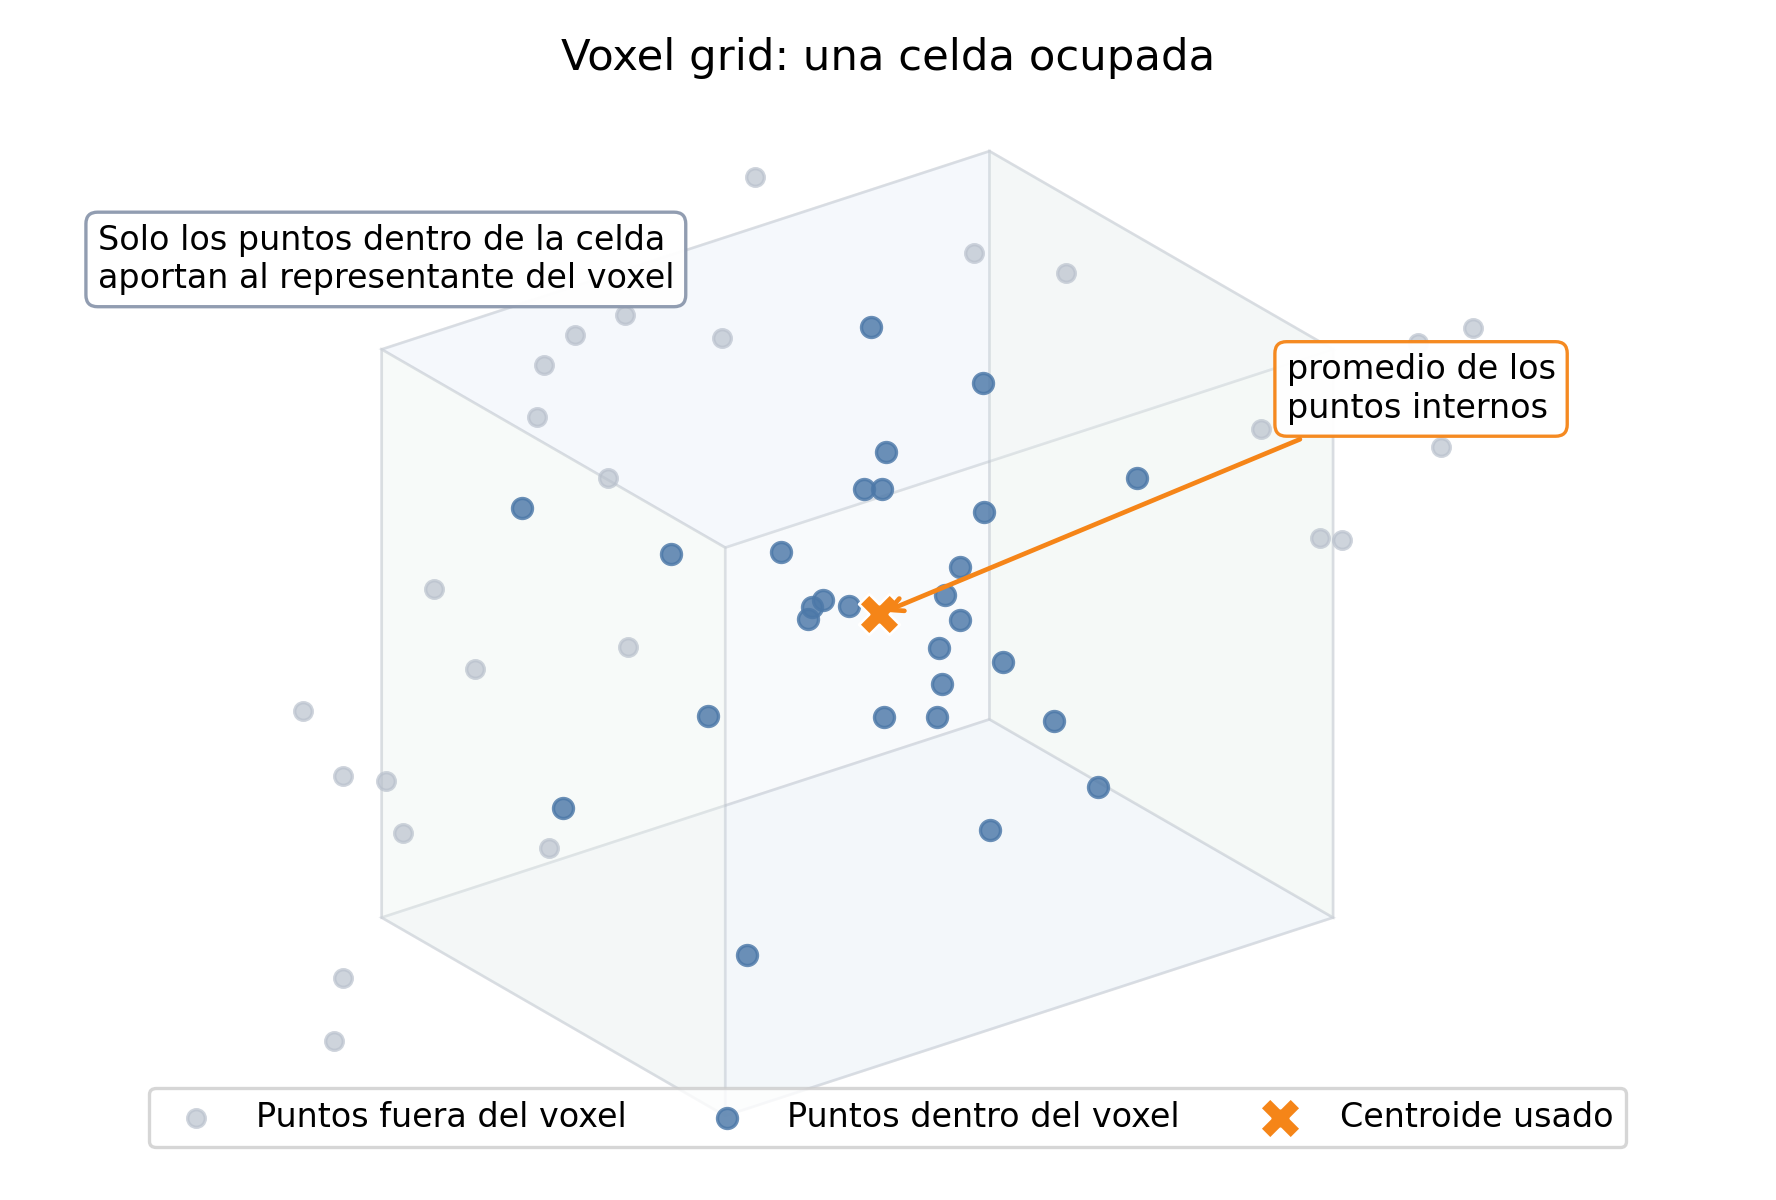
\includegraphics[width=0.88\textwidth]{_Imagenes/mapeo/ransac/voxel_grid_centroides_3d.png}
  \caption{Esquema tridimensional de submuestreo por \emph{voxel grid}. Los puntos originales
  dentro de cada celda ocupada se reemplazan por un único representante ubicado en el centroide
  de las muestras. Elaboración propia.}
  \label{fig:mt-voxel-grid-centroides}
\end{figure}

\subsection{RANSAC y refinamiento por mínimos cuadrados}
\label{subsec:mt-ransac}

En una escena real, el plano del suelo coexiste con obstáculos, paredes y ruido. RANSAC
(\emph{Random Sample Consensus}) estima modelos paramétricos en presencia de valores atípicos
\cite{Thrun2005}. Para planos, cada iteración muestrea tres puntos, ajusta un candidato y cuenta
inliers con distancia menor que $\varepsilon$. Si la fracción de inliers es $\rho$, la
probabilidad de fallar en $K$ iteraciones es:
\begin{equation}
  P_{\mathrm{fail}} = (1-\rho^3)^K.
  \label{eq:ransac-failure-prob}
\end{equation}
Esta relación permite controlar el compromiso entre robustez y tiempo de cómputo.

El modelo no requiere que el suelo coincida con un valor constante exacto de altura. Si el piso
presenta una pendiente moderada, el conjunto de puntos puede seguir explicándose mediante un plano
inclinado; la condición relevante para RANSAC es la distancia de cada muestra al plano candidato,
no la igualdad de una coordenada particular. La \Cref{fig:mt-ransac-plano-inliers} ilustra esta
idea sobre un corte bidimensional, usando la convención geométrica adoptada en el sistema.

\begin{figure}[ht]
  \centering
  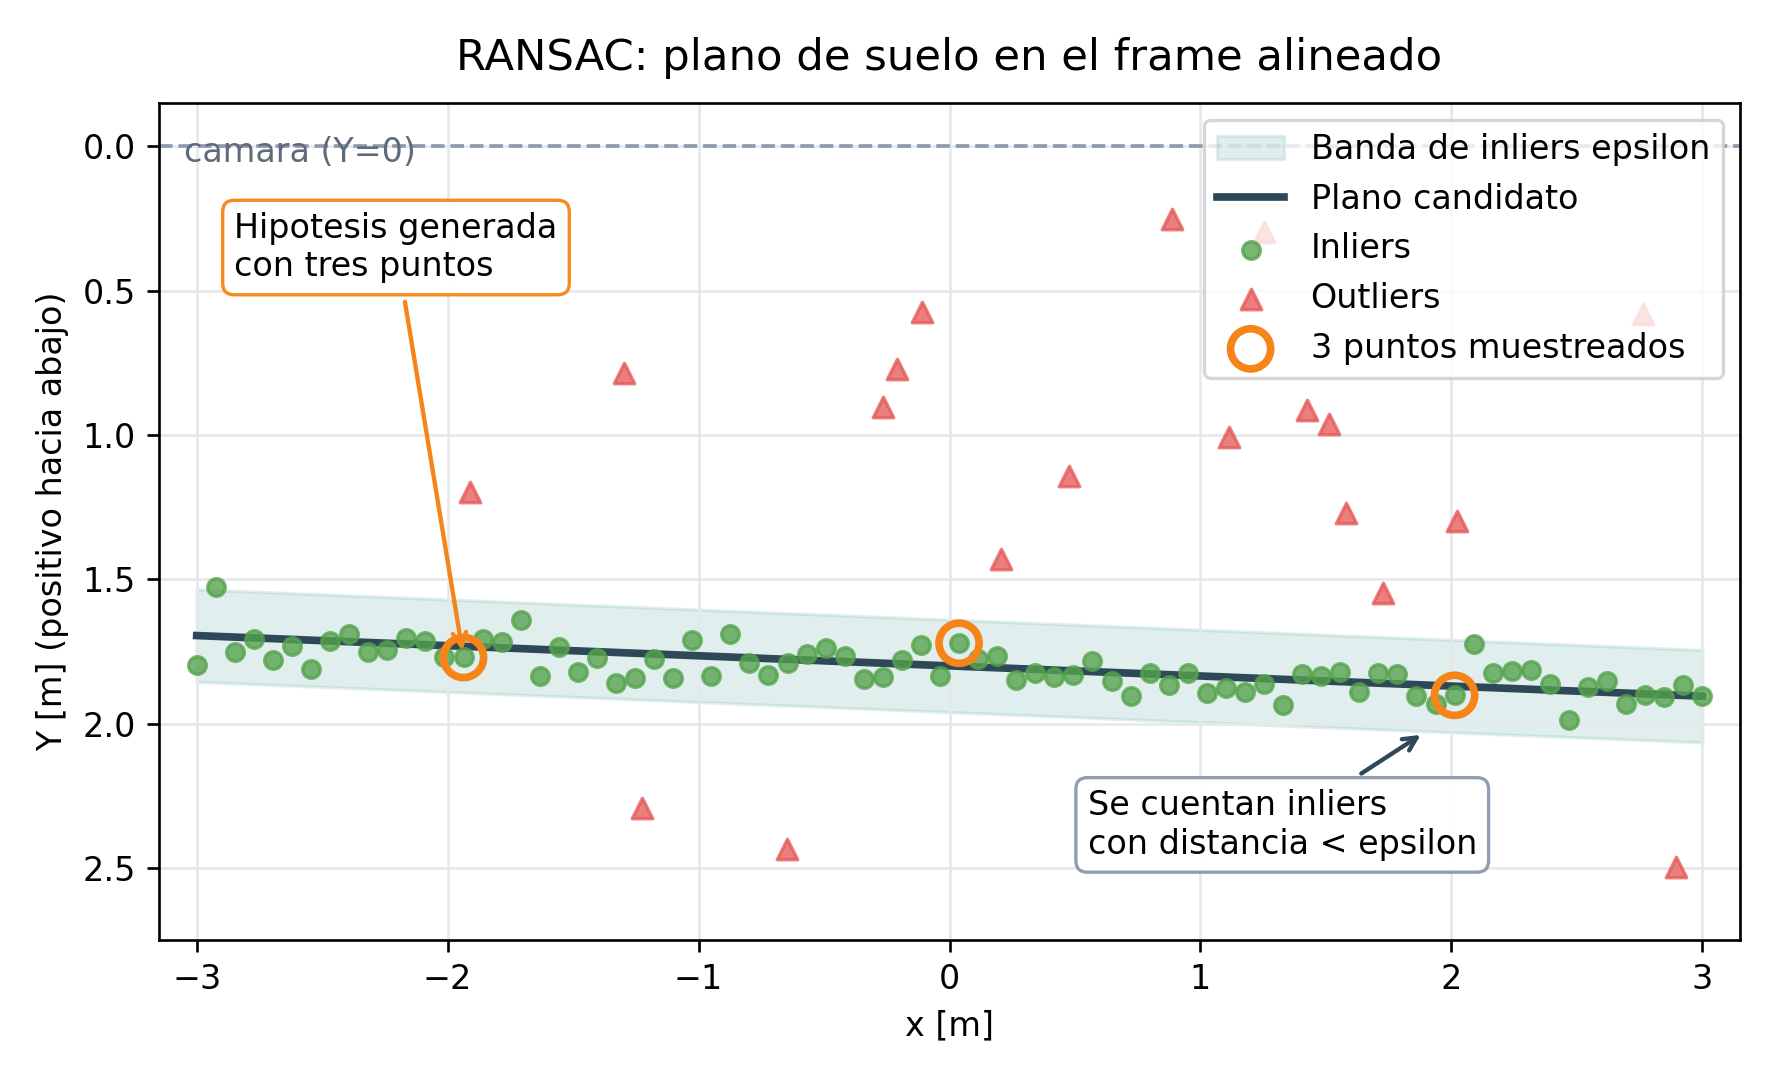
\includegraphics[width=0.88\textwidth]{_Imagenes/mapeo/ransac/ransac_plano_inliers_2d.png}
  \caption{Esquema bidimensional de RANSAC para ajuste de planos. Cada hipótesis se genera a partir
  de tres puntos y luego se cuentan como \emph{inliers} las muestras cuya distancia al plano
  candidato es menor que la tolerancia $\varepsilon$. Elaboración propia.}
  \label{fig:mt-ransac-plano-inliers}
\end{figure}

Luego de seleccionar los inliers, el plano se refina por mínimos cuadrados. Se minimiza:
\begin{equation}
  J(\mathbf{n},d) =
  \sum_{i=1}^{n}\left(\mathbf{n}^T\mathbf{p}_i+d\right)^2.
  \label{eq:ls-objective}
\end{equation}
Derivando respecto de $d$ se obtiene el centroide:
\begin{equation}
  \bar{\mathbf{p}} = \frac{1}{n}\sum_{i=1}^{n}\mathbf{p}_i,
  \qquad
  d^*=-\mathbf{n}^T\bar{\mathbf{p}}.
  \label{eq:centroid}
\end{equation}
El problema se reduce a hallar la dirección de menor varianza de la matriz de covarianza:
\begin{equation}
  C=\frac{1}{n}\sum_{i=1}^{n}
  (\mathbf{p}_i-\bar{\mathbf{p}})
  (\mathbf{p}_i-\bar{\mathbf{p}})^T.
  \label{eq:covariance}
\end{equation}
La normal óptima es el autovector asociado al menor autovalor \cite[App.~A4]{Hartley2004}:
\begin{equation}
  \mathbf{n}^*=\mathbf{q}_3,
  \qquad
  d^*=-{\mathbf{n}^*}^T\bar{\mathbf{p}}.
  \label{eq:plane-d}
\end{equation}
Para matrices $3\times3$ simétricas, el cálculo puede realizarse mediante iteraciones de
Jacobi. Cada iteración aplica una rotación ortogonal $R_{ij}(\theta)$:
\begin{equation}
  C_{k+1}=R_{ij}(\theta)^T\,C_k\,R_{ij}(\theta),
  \label{eq:jacobi-rotation}
\end{equation}
con:
\begin{equation}
  \theta =
  \frac{1}{2}
  \operatorname{atan2}\!\left(2(C_k)_{ij},(C_k)_{ii}-(C_k)_{jj}\right).
  \label{eq:jacobi-angle}
\end{equation}

\subsection{Robustez ante suelo parcialmente visible}
\label{subsec:mt-ground-robustness}

Cuando la cámara apunta al frente, el suelo puede ocupar una fracción pequeña de la nube.
Una métrica de calidad respecto del total de puntos penalizaría escenas donde el piso es
visible solo en una banda inferior. Para resolverlo se restringe el muestreo a una banda
candidata:
\begin{equation}
  \mathcal{B} =
  \left\{i:\;Y^*-\delta_l\leq Y_i\leq Y^*+\delta_h\right\},
  \label{eq:floor-band}
\end{equation}
donde $Y^*$ se obtiene mediante un histograma de alturas. La calidad se calcula en relación
con esa banda:
\begin{equation}
  \rho =
  \frac{|\text{inliers}\cap\mathcal{B}|}{|\mathcal{B}|}.
  \label{eq:relative-quality}
\end{equation}
Además, como el error axial del D435 crece con la distancia \cite{IntelRealSenseDepthTuning},
la tolerancia puede variar por punto:
\begin{equation}
  \varepsilon_i =
  \max\left(\varepsilon,\;k\lVert\mathbf{p}_i\rVert\right).
  \label{eq:variable-tol}
\end{equation}
Con este criterio, el plano no se estima a partir de toda la nube por igual. La búsqueda se
concentra en la región donde es esperable observar el piso y evalúa la calidad dentro de esa
región, incorporando además una tolerancia compatible con el ruido de profundidad.

% ---------------------------------------------------------------
\section{Fundamentos de la versión v2: odometría, mapa local y conciencia espacial}
\label{sec:mt-v2}

La versión v2 parte de la percepción filtrada alcanzada en v1 y agrega memoria espacial para cubrir
su principal limitación restante. Para que un obstáculo siga influyendo cuando abandona
el campo frontal, las observaciones locales deben transformarse a un marco común, actualizar
una grilla de ocupación y evaluarse junto con la velocidad del usuario. En la configuración
final, esta etapa se apoya en \texttt{imu\_filter\_madgwick}, \texttt{rtabmap\_odom},
\texttt{local\_mapper} y
\texttt{spatial\_awareness}.

\subsection{Filtro de Madgwick para orientación IMU}
\label{sec:mt-madgwick}

La incorporación de Madgwick corresponde a v2, no a v1. En v1 la señal inercial relevante es
el acelerómetro, porque permite estimar la vertical local a partir de la gravedad con bajo
costo. En v2, en cambio, la odometría necesita una orientación IMU filtrada que combine
acelerómetro y giróscopo. El driver de la D435i publica mediciones inerciales, pero la
orientación del mensaje IMU no constituye por sí misma una orientación filtrada utilizable por
odometría.

El problema es que ninguna de las dos mediciones inerciales resuelve por sí sola la orientación
de forma robusta. El giróscopo describe bien los cambios rápidos de orientación, pero su
integración acumula deriva. El acelerómetro, en cambio, ofrece una referencia de baja
frecuencia asociada a la gravedad, útil para corregir roll y pitch cuando la aceleración
dinámica no domina la medición \cite{Woodman2007}. Esta complementariedad motiva el uso de
un filtro que propague la orientación con el giróscopo y la corrija con la dirección de
gravedad medida por el acelerómetro.

Para este propósito se usa el filtro de Madgwick \cite{Madgwick2010}. La propagación por
giróscopo puede
escribirse como:
\begin{equation}
  \dot{q}_{\omega} =
  \frac{1}{2}\,q\otimes(0,\boldsymbol{\omega}),
  \label{eq:quat-gyro-prop}
\end{equation}
donde $\boldsymbol{\omega}$ es la velocidad angular medida. La corrección ajusta el
cuaternión para reducir el error entre la gravedad medida y la gravedad esperada. En este
sistema se deshabilita el magnetómetro, por lo que el filtro aporta principalmente una
estimación estable de roll y pitch para inicializar y regular \texttt{rgbd\_odometry}. La
corrección de la deriva horizontal proviene de la odometría visual.

La elección de Madgwick responde a que ofrece una estimación de orientación de bajo costo por
muestra, adecuada para ejecución embebida. Además, la implementación utilizada produce un
cuaternión válido en
\texttt{/imu/data\_filtered}, requerido por \texttt{rgbd\_odometry} cuando se configura con
inicialización por IMU.

\subsection{Odometría RGB-D con RTAB-Map}
\label{sec:mt-vio}

La odometría visual estima el movimiento de la cámara a partir de cambios entre fotogramas
consecutivos \cite{Hartley2004}. En v2 se utiliza \texttt{rgbd\_odometry} del paquete RTAB-Map
\cite{Labbe2019RTAB}. El nodo consume imagen RGB, parámetros intrínsecos, profundidad alineada a
color y la IMU filtrada. La profundidad convierte el problema visual en una estimación
métrica, mientras que la IMU aporta una orientación inicial y una predicción útil ante
movimiento rápido.

RTAB-Map puede operar como biblioteca de SLAM y mapeo, pero en este sistema se usa su
odometría RGB-D como fuente local de pose. La salida se publica como
\texttt{nav\_msgs/Odometry} y se remapea a \texttt{nav\_odom}. El marco \texttt{odom} no
representa un sistema global absoluto; es un marco local continuo, con origen definido al
inicio de la ejecución y con deriva acumulada a largo plazo. Esta propiedad es suficiente para
un mapa local de corto alcance, porque la coherencia requerida abarca segundos y metros
recientes, no un mapa permanente de todo lo recorrido previamente.

\subsection{Marcos de referencia y convención REP-103}
\label{sec:mt-frames}

ROS define convenciones estándar de unidades y marcos en REP-103 \cite{REP103}. Sin embargo,
los flujos ópticos de cámara utilizan una convención natural para imágenes: $x$ hacia la
derecha, $y$ hacia abajo y $z$ hacia adelante. El sistema combina ambas perspectivas: RTAB-Map
publica odometría en sus marcos ROS, mientras que el pipeline geométrico interno trabaja con
la convención óptica de la cámara.

La transformación entre convenciones no altera la información física; solo expresa la misma
pose en ejes compatibles con la grilla local. Para el mapa 2D se conserva la posición
horizontal del sensor y el yaw extraído de la orientación. Roll y pitch no se aplican en esta
etapa porque la nube ya fue alineada con gravedad en v1. Esta separación evita mezclar la
estabilización vertical de la percepción con la acumulación horizontal del mapa.

\subsection{Sincronización temporal de observaciones y odometría}
\label{sec:mt-sync}

El mapa local combina tres fuentes temporales: nube de obstáculos, extremos de rayos libres y
odometría. Las dos nubes derivan del mismo frame de profundidad, por lo que comparten
\texttt{header.stamp} y pueden sincronizarse con política exacta. La odometría, en cambio, llega a
otra frecuencia; por eso se mantiene un buffer y se toma la muestra más reciente no posterior
al instante de la observación.

Esta política evita usar una pose futura respecto del frame de profundidad y reduce
inconsistencias geométricas. Si no hay odometría disponible, el frame se descarta para no
insertar puntos en una posición arbitraria. El criterio prioriza coherencia espacial sobre
completitud de frames, decisión adecuada para un mapa local reactivo.

\subsection{Representaciones espaciales locales}
\label{sec:mt-local-maps}

Se distingue entre mapas globales, que buscan representar un entorno completo, y mapas locales
de corto alcance, centrados en el usuario y limitados a una ventana espacial. Los mapas locales
permiten actualizaciones frecuentes con baja latencia, por lo que son adecuados para evasión
reactiva \cite{brock1999high,macenski2020nav2}. En este trabajo se adopta una grilla de
ocupación 2D local en el marco \texttt{odom}.

La grilla local se expresa en el plano horizontal. La altura estimada de la cámara respecto
del suelo, publicada por el filtro geométrico, se usa para ubicar correctamente el origen de
la visualización y mantener consistencia entre la nube 3D, el plano de suelo y la
representación 2D.

\subsection{Grillas de ocupación y log-odds}
\label{sec:mt-occupancy-grid}

La grilla de ocupación fue introducida por Elfes \cite{Elfes1989} como una discretización
probabilística del espacio. Cada celda $m_i$ almacena la probabilidad de ocupación
condicionada al historial de observaciones $z_{1:t}$. Para actualizar eficientemente se usa la
escala de
\emph{log-odds}:
\begin{equation}
  l_t(m_i) =
  l_{t-1}(m_i) +
  \underbrace{\log\frac{P(m_i=1\mid z_t)}{P(m_i=0\mid z_t)}}_{l_{\text{sensor}}(z_t,m_i)}
  - l_0.
  \label{eq:log-odds-update}
\end{equation}
La ecuación~\ref{eq:log-odds-update} convierte la actualización bayesiana recursiva en una
suma
\cite{Thrun2005}. Las celdas impactadas por obstáculos reciben un incremento positivo
$l_{\text{occ}}$, mientras que las celdas atravesadas por rayos libres reciben un incremento
negativo $l_{\text{free}}$. Para estabilidad numérica, $l_t$ se satura en
$[l_{\min},l_{\max}]$.

La probabilidad puede recuperarse como:
\begin{equation}
  P(m_i=1\mid z_{1:t}) =
  1-\frac{1}{1+\exp(l_t(m_i))}.
  \label{eq:log-odds-prob}
\end{equation}
Esta forma permite publicar la grilla en \texttt{nav\_msgs/OccupancyGrid}, cuyo rango habitual
representa ocupación entre 0 y 100.

\subsection{Ray casting con Bresenham}
\label{sub:bresenham}

Además de marcar ocupada la celda del obstáculo, el mapa debe marcar como libre el espacio
atravesado por el rayo de medición. Para ello se usa el algoritmo de Bresenham
\cite{Bresenham1965}. Dado un origen $(x_0,z_0)$ y un destino $(x_1,z_1)$ en coordenadas
enteras de celda, el algoritmo avanza sobre el eje dominante y decide cuándo incrementar el
eje subordinado mediante una variable de error acumulado. Así recorre las celdas intersectadas
por el segmento sin calcular intersecciones en punto flotante.

En este sistema se aplican dos tipos de rayos. Los rayos con obstáculo marcan libres las
celdas intermedias y ocupada la celda final. Los rayos asociados a suelo, techo o mediciones
sin obstáculo dentro del rango marcan libre también el extremo final. Para no borrar
evidencia acumulada de forma excesiva, una celda recibe evidencia libre como máximo una vez
por frame.

\subsection{Ventana local deslizante y olvido espacial}
\label{sec:mt-sliding-window}

La memoria espacial se mantiene en una ventana finita. Cuando la odometría indica
desplazamiento del sensor, la grilla se desplaza una cantidad entera de celdas y las celdas
nuevas se reinicializan con prior neutro. Para evitar pérdida de resolución a bajas
velocidades, los desplazamientos sub-celda se acumulan hasta superar el tamaño de celda.

Además del corrimiento de ventana, se emplea un radio de olvido local: las celdas demasiado
alejadas del sensor vuelven al prior. Este mecanismo impide que observaciones viejas dominen
indefinidamente y mantiene el mapa enfocado en la región útil para navegación inmediata.

\subsection{Filtrado espacial y temporal}
\label{sec:mt-spatiotemporal-filtering}

El filtrado espacial aparece en dos niveles. Primero, la reducción a \texttt{DepthGrid} resume
múltiples muestras en celdas. Segundo, la grilla de ocupación acumula evidencia por celda en
el plano local. El filtrado temporal surge de la actualización log-odds: observaciones
persistentes refuerzan ocupación y mediciones libres repetidas la reducen. Este comportamiento
suaviza detecciones esporádicas, aunque requiere saturación y olvido para evitar que el mapa
se vuelva rígido frente a cambios reales. En la implementación actual no se aplica un
decaimiento explícito por edad de celda: una ocupación pierde peso cuando es contradicha por
rayos libres, cuando queda fuera del radio local o cuando sale de la ventana deslizante.

\subsection{Conciencia espacial y tiempo hasta colisión}
\label{sec:mt-spatial-awareness}

La capa de conciencia espacial evalúa riesgos fuera del campo frontal ya comunicado por la
grilla háptica. Primero decodifica celdas ocupadas por encima de un umbral y agrupa
componentes conectadas por vecindad. El agrupamiento elimina ruido aislado: una celda ocupada
solitaria no necesariamente representa un obstáculo físico relevante.

Para cada celda candidata se calcula su posición relativa respecto de la pose del usuario y se
descarta si cae dentro del campo frontal ya cubierto. Luego se evalúa si intersecta el
corredor corporal y si existe velocidad de cierre suficiente. El tiempo hasta colisión se
define como:
\begin{equation}
  t_{\text{tc}} = \frac{d}{v_c},
  \label{eq:ttc}
\end{equation}
donde $d$ es la distancia al obstáculo y $v_c$ la componente de velocidad dirigida hacia él.
La ecuación~\ref{eq:ttc} prioriza urgencia dinámica, no solo proximidad geométrica. La
intensidad asociada puede escalarse linealmente entre un tiempo mínimo y un horizonte máximo:
\begin{equation}
  I_{\text{riesgo}} =
  100\,
  \operatorname{sat}_{[0,1]}
  \left(
    \frac{t_{\max}-t_{\text{tc}}}{t_{\max}-t_{\min}}
  \right).
  \label{eq:risk-intensity}
\end{equation}
Los riesgos se clasifican en izquierda, derecha y posterior. En cada región se conserva el
candidato más urgente, con histéresis sobre velocidad de cierre para evitar conmutaciones
rápidas alrededor del umbral.

\subsection{Fusión háptica con riesgo contextual}
\label{sec:mt-haptic-fusion}

En v2, la salida háptica ya no representa únicamente la percepción frontal instantánea. La
grilla frontal sigue codificando distancia a obstáculos en el campo visual, mientras que la
conciencia espacial aporta señales semánticas de riesgo lateral y posterior. La fusión se
realiza por máximo de intensidad: si una celda ya está activa por percepción frontal, una
señal contextual solo la aumenta si su intensidad es mayor.

Esta regla conserva la interpretación de seguridad de la interfaz. El usuario recibe siempre
la señal más urgente entre percepción inmediata y memoria contextual, sin promediar señales
que representan fenómenos distintos.

\subsection{Métricas de evaluación para percepción y mapeo}
\label{sec:mt-metrics}

Las métricas de evaluación siguen el orden incremental v0--v1--v2. En v0 se evalúan latencia
\emph{end-to-end}, tasa de publicación, coherencia entre distancia e intensidad y costo de
transmisión UART. En v1 se agregan error geométrico respecto del plano de suelo, estabilidad
de la altura de cámara, tasa de falsos positivos por suelo o techo y costo computacional del
filtrado geométrico. En v2 se evalúan precisión y recall de la grilla local, estabilidad
temporal por celda, vigencia de odometría, cobertura de riesgo lateral y posterior, y consumo
de CPU y memoria. Esta organización conecta la teoría con los bloques experimentales y evita
mezclar métricas de capacidades que aparecen en versiones distintas.
